\chapter{Results}
\label{chapter:results}

In this chapter we present how the front-end application works from the user's standpoint and how the React components mutate upon browser events. In section \labelindexref{UI overview}{sec:ui-overview} we present how the UI looks and how its structured after the components are rendered.

Next, in section \labelindexref{Edit Panel}{sec:edit-panel} we describe how the \texttt{GenericForm} components generate edit panels and how they are displayed.

Finally in the \labelindexref{Panel Nesting}{sec:panel-nesting} section we describe how the application renders the explored content trough the API.

\section{UI overview}
\label{sec:ui-overview}



\begin{sidewaysfigure}	
	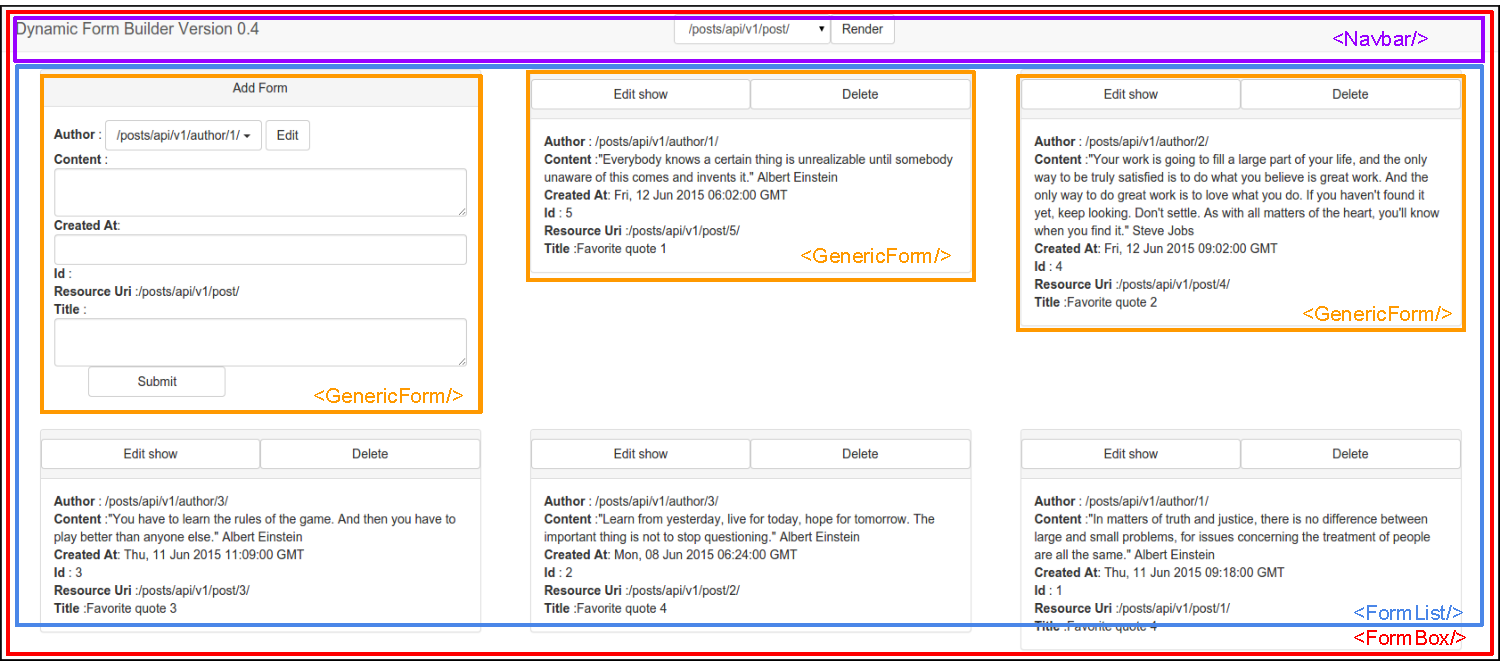
\includegraphics[scale=0.90]{src/img/screenshot-app-0.pdf}
	\label{img:main-view}
	\caption{Main view app}
\end{sidewaysfigure}


\section{Edit Panel}
\label{sec:edit-panel}

\fig[scale=0.55]{src/img/panels2.pdf}{img:panels}{PANELS}


\subsubsection{Add Panel}
\label{sec:add	-panel}

\fig[scale=0.5]{src/img/add-panel.png}{img:add-panel}{Add panel component}

\section{Panel Nesting}
\label{sec:panel-nesting}

\fig[scale=0.50]{src/img/nesting2.pdf}{img:nesting}{PANELS}